\documentclass[12pt]{article}
\setcounter{secnumdepth}{0}

\usepackage{txfonts}
\usepackage{setspace}
\usepackage{xcolor}
\usepackage{titlesec}
\usepackage[left=1in, right=0.59in, top=0.79in, bottom=0.79in]{geometry}
\usepackage{graphicx}
\usepackage{float}
\usepackage[utf8x]{inputenc}

\setstretch{1.15}
\definecolor{sectioncolor}{RGB}{0,102,204}

\titleformat{\section}[block]{\color{sectioncolor}\bfseries\large}{}{0pt}{}


\begin{document}

\begin{center}


	\begin{figure}[h!]
		\centering
		
\includegraphics[width=0.5\textwidth]{assets/images/banm.png}
		
	 \end{figure}


	
{\fontsize{14pt}{14pt}\selectfont

\textbf{PipeUp project}

}	

\end{center}

Rovshan Khalilov,
Kifayat Gambarova, 
Sevinj Mollayeva,
Fuad Gafarli,
Murad Feyzullayev

\begin{center}
	Department of Chemical Engineering, BHOS, Azerbaijan

	EACOP; Pipeline route; Pressure; Aspen HYSYS
\end{center}
\newpage
\tableofcontents
\newpage
\section{Abstract}
{\fontsize{12pt}{12pt}\selectfont



\hspace*{1em} Initially, the Human Rights Due Diligence Report is one type of enterprises from the EACOP, that shows its commitments and visible assumptions which are related to civil liberties respect. Since Human Rights Impact Assessment was initiated by EACOP, it observed an increased request from the firms to represent the analysis of human rights via the principles of business and civil rights in the United Nations organizations. So, the expectations for Human Rights Due Diligence (HRDD) encloses more strict directives from the states, encompassing policies and laws forcing companies to attend in the HRDD. What is more, there is a big attention from the people who are able to invest much and financial institutions, including HRDD into their evaluation of some invested projects, such as social, environmental and governmental. In addition to this, it can be clearly seen that, there is a big role of civil society of organizations in terms of supporting and to sustaining scrutiny. 
\\

To conclude this part, it can be said that the mentioned expectations may make necessary companies to integrate the HRDD in terms of regular business operations, can bring attention to continual application rather than occasional examination. Hence, except for revision of HRIA which was conducted in 2017-2018, this project report also illustrates the establishment of EACOP project and implementation of system management for continuous HRDD. In other words, it explains that how the company should deal with civil rights issues, when the project is going to be applied.  
\\

Considering that there is a big focus on the EACOP project, it confirms its dedication to transparency, and promises to be willing to report and discuss the main problems that are related to human rights. This project report underlines that the elements of communication as crucial elements within EACOP’s continual HRDD process. Meanwhile, these elements give a chance to incline the awareness about the integration of business and civil rights in Tanzania and Uganda. Lastly, there are a few examples of projects or companies which obey the rules of HRDD process.
\\
\\

}
\section{Introduction}

{\fontsize{12pt}{12pt}\selectfont 

\hspace*{1em}Total East Africa Midstream B.V carried out the Environmental Social Impact Assessment for the EACOP project, submitting the Environmental and Social Impact Assessment report to the National Environment Management Authority in order to revise on 15th January 2019. In 1998, the regulation of NEIA, a copy of ESIA report had been sent to the Uganda Petroleum Authority for obtaining feedback and examination. After 21 years, UPA have sent feedback and comments to the NEMA, on o9th April 2019. Additionally, the UPA attended technical assessment of the Environmental Social Impact Assessment report which was carried out by NEMA from 30th June to 5th July 2019 by means of other Government Ministries, Agencies and Departments. The extra MDAs included in the process were Uganda Wildlife Authority, Ministry of agriculture and lands, energy and mineral night, Housing and Urban development, directorate of environment affairs and water resource management, and the district local government.
\\

In 1995, RSK and Eco Consults Ltd, carried out the ESIA for the EACOP project with the Group 19 of the NEA from the side of TEAM, and after 3 years with the EIA. So, this project report is aimed at giving more detailed information about the EACOP project and ecological and social aspects and decide according to the mentioned information. 
\\

Finally, NEMA was marked as NEMA/4.5.5 through a letter on 20th September 2019 and PAU was instructed to organize the public hearings for EACOP project in 1998, also other projects which have transboundary influences and is controversial.  
\\
\\

}


\section{Problem Statement}

{\fontsize{12pt}{12pt}\selectfont  

\hspace*{1em}It is obvious that the East African Crude Oil Project has multiple benefits, including addressing energy poverty, improving the lives of the local inhabitants, also mitigating unemployment since it is aimed to recruit workers from the local communities. However, the project is accompanied by severe negative outcomes, comprising environmental, social, and climatic risks. One of the most detrimental impacts is that a number of residential areas, and social infrastructures, such as houses, hospitals, schools, etc. are destroyed as a result of the building of the pipeline. Therefore, this prompts questions and discontent about the implementation of this project.
\\

The potential environmental risks are also one of the negative consequences. Ecosystems and protected areas are disrupted. Because of oil spills, land and water contamination risks are inevitable. This raises an alarm that the lives of people, fauna, and flora of the environmental ecosystems are threatened and potentially in danger. This kind of hazards can lead to prolonged unfavorable outcomes related to the livelihood of the population and biodiversity.
\\

From the perspective of social impacts, as a result of the EACOP project, thousands of people from the local communities are displaced from their lands and houses. This mandatory displacement can lead to conflicts between the adversely impacted people and the company.  In order to mitigate this problem, 45,000,000 USD have been allocated to the population of Uganda. This fund covers monetary compensation, costs of relocation and resettlements, and other types of support. However, by not disrupting local communities, approximately more than 90 million USD can be saved[1].
\\


}


\begin{figure}[h!]
\begin{center}

	\centering
	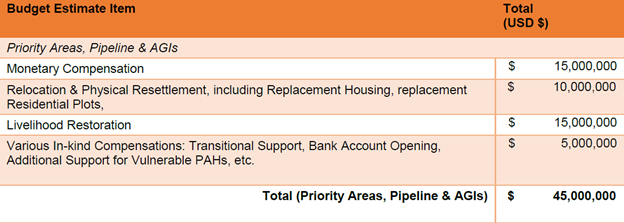
\includegraphics[width=0.7\textwidth]{assets/images/table.png}
	
	\textit{Table 1}
\end{center}
	
\end{figure}

{\fontsize{12pt}{12pt}\selectfont  
\hspace*{1em} Because of the issues presented above, in our project, route of the pipeline does not cross any problematic areas (protected areas, lakes, hospitals, schools, houses and so on). As a result, our route is longer than real route. Google Earth Pro was used to determine buildings, while maps and articles were used for protected areas [2]. Additionally, there is a problem with changes in elevation which has drastic effect on the pressure inside of the pipe. This complication was solved with the help of Google Earth Pro also.
\\

In order to increase the rate of the flow some pump stations are used, however after some point it is necessary to decrease the flow of oil. So, Pressure Reduction Stations are used to drop pressure - valves are used in our project [3].  In addition, with the help of Aspen HYSYS pressure drops due to elevation and pipeline length is defined. After defining this pressure drops, the location of pump stations and power of pumps are identified.
\\

}

\section{Methodology}

{\fontsize{12pt}{12pt}\selectfont  
\hspace*{1em} With the purpose of minimizing such potential risks of the EACOP, our team's approach was to redesign the trajectory of the pipeline with the assistance of Google Earth Pro. It is significant to note that by considering the welfare of the local communities, houses, hospitals, churches, schools, and other residential and social infrastructures are not destroyed. That being said, the trajectory of the pipeline is increased to 1500.2km. 
\\

For Pressure Reduction stations the equipment illustrated on 1st Picture is utilized. This piece of equipment consists of 4 valves which are divided into 2 sections: 2 valves on the right side and 2 on the left side. The division of valves is done in order to decrease the flow for one valve, which results in better overall safety of the process since the reduction of pressure is easier this way. The type of valves used in the apparatus is control valves.
\\




}



\begin{figure}[h!]
	\centering
	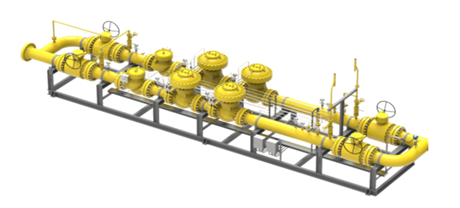
\includegraphics[width=0.7\textwidth]{assets/images/pressure_reduction_station.png}
	\caption{\textit{Pressure Reduction Station}}
	
 \end{figure}


 {\fontsize{12}{12}\selectfont 
	\hspace*{1em} After that, the necessary calculations regarding pressure are conducted by means of Excel software. Additionally, the pump locations and overall, the entire project are designed through Aspen HYSYS software.  We also contacted many professional engineers from the Petroleum and Chemical Engineering disciplines as well as local and international companies to determine the suitable pipe material, and further calculate and determine the necessary costs.
 	\\

 }

 


\section{Application and Results}
{\fontsize{12}{12}\selectfont 
The crude oil of Uganda is significantly high in wax content prompting being highly viscous and in a solid phase at room temperature. Therefore, to transport it, the temperature along the entire length of the pipeline must be maintained at 50°C underscoring industrial intricacies dealing with such viscous crude oil[4]. Notwithstanding its difficult properties, the oil of Uganda is classified as "sweet” due to having low acidic content which induces it to appeal to the international market[5]. 
\\

Uganda's oil has unique characteristics with an API gravity of 17°C-33°C which highlights being categorized as medium to heavy in density. It has a significantly low sulfur content which makes it more convenient due to the fact that it is combusted with air, the amounts of toxic releases will be low, and the corrosion of the pipeline material will be minimized from the economic and environmental perspectives.
\\

The meticulous calculations regarding pressure drop throughout the pipeline are needed to ensure the safety and sustainability of the design of the system, additionally, from an economic and environmental point of view, efficiency and obtained head losses are considered. The determination of the number of pumps in order to achieve the best possible performance is involved by emphasizing decreasing head loss due to friction. To achieve successful results, it is needed to conduct calculations of the key parameters, such as the density and viscosity of Uganda's oil. Taking into account that significant discrepancies may lead to undesirable outcomes, the accuracy of these figures is paramount. It is aimed to transport a quantity of 216,000 barrels of oil per day from Uganda to Tanzania.
\\

To define the viscosity value, necessary computations are carried out as shown in Table 2[6][7].

\begin{table}[H]
	% \centering
	\begin{tabular}{|c|c|c|c|c|c|c|c|c|c|c|}
	  \hline
	  \textbf{Components} & \textbf{A} & \textbf{B} & \textbf{C} & \textbf{D} & \textbf{log(viscosity)} & \textbf{viscosity calc.} & \textbf{mass fraction} \\
	  \hline
		N2 & 42.61 & 0.475 & -0.000099 & 0 & - & 185.706429 & 0.001 \\
		\hline
		CO2 & 11.81 & 0.497 & -0.00011 & 0 & - & 160.86481 & 0.004 \\
		\hline
		H2S & 6.545 & 0.424 & -2.85714E-06 & 0 & - & 143.198917 & 0.005 \\
		\hline
		CH4 & 3.844 & 0.402 & -0.000142 & 0 & - & 118.875282 & 0.05 \\
		\hline
		C2H6 & 0.513 & 0.335 & -0.0000712 & 0 & - & 101.289775 & 0.03 \\
		\hline
		C3H8 & -5.461 & 0.326 & -0.000108 & 0 & - & 88.569468 & 0.04 \\
		\hline
		C4H10 & -6.857 & 673.9 & 0.022 & -0.000031 & -0.86752 & 0.1356679 & 0.05 \\
		\hline
		C7H16 & -5.778 & 805.9 & 0.013 & -0.000015 & -0.64888856 & 0.224445778 & 0.05 \\
		\hline
		C6H14 & -5.073 & 655.4 & 0.012 & -0.000018 & -1.02495403 & 0.09441608 & 0.02 \\
		\hline
		Heavy oil & & & & & & 1200000 & 0.6 \\
		\hline
		\multicolumn{2}{|c|}{\textbf{Ttemperature(K)}} & 323 & \multicolumn{3}{|c|}{\textbf{total dynamic viscosity(μP)}} & \multicolumn{2}{|c|}{720014.1936} \\
		\hline
		\multicolumn{6}{|c|}{\textbf{Total dynamic viscosity (Pa*s)}} & 
		\multicolumn{2}{|c|}{0.072001419} \\
		\hline
	\end{tabular}
	\begin{center}
	\textit{Table 2}
	\end{center}
	% \caption{Your Table Caption}
	% \label{tab:your_table_label}
  \end{table}

}

{\fontsize{12pt}{12pt}\selectfont 
\hspace*{1em} The Table 3 shows the calculated value for the density of the Uganda’s crude oil.
}


\begin{table}[H]
	\centering
	\begin{tabular}{|c|c|c|c|c|c|c|c|}
	  \hline
	  \textbf{Components} & \textbf{A} & \textbf{B} & \textbf{n} & \textbf{Tc} & \textbf{T} & \textbf{density} & \textbf{Mass fraction} \\
	  \hline
	  N2 & 0.31205 & 0.28479 & 0.2925 & 126.1 & 323 & 175.83 & 0.001 \\
	  \hline
	  CO2 & 0.46382 & 0.2616 & 0.2903 & 304.19 & 323 & 452.79 & 0.004 \\
	  \hline
	  H2S & & & & & & 14.2 & 0.005 \\
	  \hline
	  CH4 & 0.15998 & 0.2881 & 0.277 & 190.58 & 323 & 125.91 & 0.05 \\
	  \hline
	  C2H6 & 0.20087 & 0.2733 & 0.2833 & 305.42 & 323 & 196.67 & 0.03 \\
	  \hline
	  C3H8 & & & & & & 500 & 0.04 \\
	  \hline
	  C4H10 & 0.22827 & 0.2724 & 0.2863 & 425.18 & 323 & 541.94 & 0.05 \\
	  \hline
	  C7H16 & 0.23237 & 0.2602 & 0.2791 & 540.26 & 323 & 660.1 & 0.05 \\
	  \hline 
	  Heavy oil & & & & & 323 & 970 & 0.6 \\
	  \hline
	  H2O & 0.3471 & 0.274 & 0.28571 & 647.13 & 323 & 1004.4 & 0.15 \\
	  \hline
	  C6H14 & 0.23242 & 0.265 & 0.2781 & 507.43 & 323 & 633.2 & 0.02 \\
	  \hline
	  \multicolumn{6}{|c|}{Total density of mixture ($kg/m^3$)} & \multicolumn{2}{|c|}{840} \\
	  \hline
	\end{tabular}
	\begin{center}
	\textit{Table 3}
	\end{center}
	
  \end{table}

  {\fontsize{12pt}{12pt}\selectfont 

  Since the density and viscosity are obtained, head loss can be determined:
  }

  \begin{table}[H]
	\centering
	\begin{tabular}{|c|c|c|}
	  \hline
	  \textbf{Parameters} & \textbf{Values} & \textbf{Units} \\
	  \hline
		\textbf{Diameter} & 0.6 & $m$\\
	  \hline
	  \textbf{Length} & 1500.2 & $km$ \\
	  \hline
	  \textbf{Viscosity} & 0.072 & $Pa*s$ \\
	  \hline
	  \textbf{Density} & 840 & $kg/m^3$ \\
	  \hline
	  \textbf{Absolute roughness} & 0.046 & $mm$ \\
	  \hline
		\textbf{Relative roughness} & 7.66667E-0.5 & - \\
	  \hline
	  \textbf{Volumetric flowrate} & 0.4 & $m^3/s$ \\
	  \hline
	  \textbf{Reynolds number} & 9903.0 & - \\
	  \hline
	  \textbf{Flow velocity} & 1.415 & $m/s$ \\
	  \hline
	  \textbf{Moody friction factor} & 0.03124 & \\
	  \hline
	  \textbf{Pressure loss:} & 65658876.13 & $Pa$ \\
	  \hline
	  \textbf{Pressure loss:} & 65.658876.13 & $MPa$ \\
	  \hline
	  \textbf{Head loss:} & 7967.923418 & $m$ \\
	  \hline
	\end{tabular}
	\begin{center}
	\textit{Table 4}
	\end{center}
	
  \end{table}

  {\fontsize{12pt}{12pt}\selectfont 

  In order to identify the location of pump stations and pressure reduction stations, the elevations and the values from Aspen HYSYS are used. The route of pipeline is shown in 2nd Picture:
  \\
  
  }


\begin{figure}[H]
	
	\begin{center}
	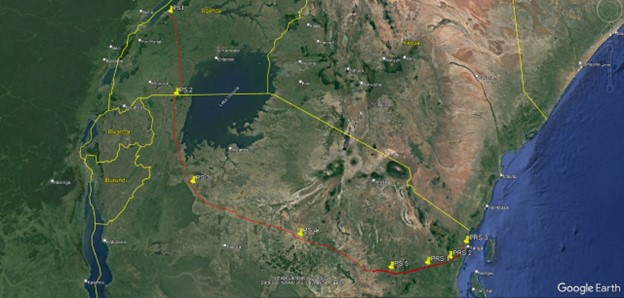
\includegraphics[width=0.7\textwidth]{assets/images/pipeline_route.jpg}
	\caption{\textit{Pipeline Route}}
	
	\end{center}
	
 \end{figure}


 {\fontsize{12pt}{12pt}\selectfont 
 While drawing simulation in Aspen HYSYS (3rd  Picture ) , firstly parameters for input have to be indicated. These parameters are components of oil, temperature, pressure, liquid flow of oil and it is illustrates in 4th Picture.
\\

}

\begin{figure}[H]
	\centering
	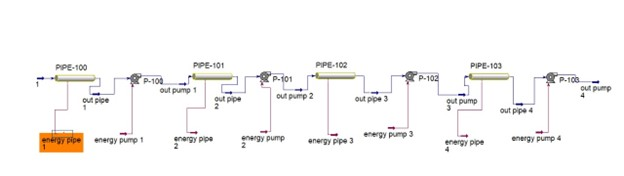
\includegraphics[width=0.7\textwidth]{assets/images/some_pipe_stuff.jpg}
	\caption{\textit{Aspen HYSYS Simulation} }

	\vspace{10mm}

	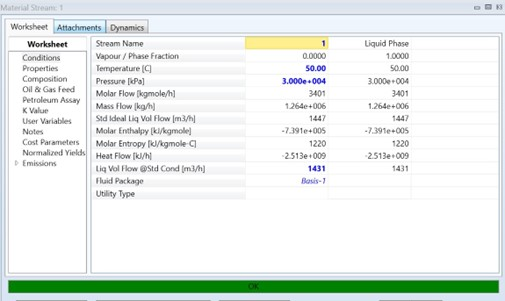
\includegraphics[width=0.7\textwidth]{assets/images/inlet.jpg}
	\caption{\textit{Conditions for inlet stream}}
	
 \end{figure}
 

{\fontsize{12pt}{12pt}\selectfont
Consequently, remaining data (for example molar flow and mass flow) is defined by Aspen HYSYS. And, for each pipeline, the length, elevation, pressure loss and the power of the pump are indicated in the table below (calculated by Aspen HYSYS). 
\\


}

\begin{table}[H]
	\centering
	\begin{tabular}{|p{3cm}|p{2cm}|p{2cm}|p{2cm}|p{2cm}|p{2cm}|}
	  \hline
	    & Length of pipeline, $km$ & Average elevation, $m$ & Pressure drop, $kPa$ & Power of pump, $kW$ & Pump Station number \\
	  \hline
	  PS1 - PS2 & 292.4 & 1197 & 5996.33 & 13110 & PS2 \\
	  \hline
	  PS2 - PS3 & 292 & 1222 & 6455 & 12950 & PS3 \\
	  \hline
	  PS3 - PS4 & 367 & 1241 & 3719 & 14700 & PS4 \\
	  \hline
	  PS4 - PS5 & 280 & 1330 & 6973 & 12800 & PS5 \\
	  \hline 
	  PS5 - PRS1 & 108 & 754 & 19169 & &  \\
	  \hline
	  PRS1 - PRS2 & 68 & 427 & 12391 & & \\
	  \hline 
	  PRS2 - PRS3 & 69.7 & 145 & 8268 & & \\
	  \hline
	  PRS3 - ST & 6.12 & 23 & 7685 & & \\
	  \hline
	\end{tabular}
	\begin{center}
	\textit{Table 5. Length, average elevation, pressure drop of each pipeline, and power of pump }
	\end{center}
	\label{tab:your_table_label}
  \end{table}


\section{Discussion}
{\fontsize{12pt}{12pt}\selectfont
\hspace*{1em}In this section, the outcomes that are shown in the Results part are discussed and some problems related to project are addressed. Firstly, the one important side goal of the project is taking environmental risks such as contamination into consideration and minimizing the social impacts which are mainly disagreement between people. To achieve these, some essential steps are taken. As shown in Methodology section, to avoid those problems, the whole pipeline trajectory was remodeled. According to new design, trajectory does not cross any houses, schools and etc. so that there is no distortion to local communities. This step increases the route to 1500.2 km to our main route; however, this alternative way saves approximately 90 million USD. Elevations across the route are considered. Although it adds extra cost to our budget, the money that is saved totally compensates it. Natural disasters, seasonal changes are mainly considered while choosing route. Route does not cross rivers to keep away from problems which are related to alterations when seasons change. The climate conditions which are extreme temperature changes, the disasters as floods, volcanic eruptions and others have to be prevented.
\\

Another important issue is about the pipeline itself. The material of the pipe should be chosen carefully and considering all the external impacts in long term. First thing that can weaken the pipeline is corrosion. The material should be resistant to harsh environments that can have soil, moisture ad etc. Material should be strong enough to endure external forces such as pressure and temperature. Another point is compatibility. Material must have compatibility with the oil inside the pipe to avoid the chemical reactions that can make problems for the coherence of pipeline. As mentioned in Results part, Uganda oil has difficult properties. So, the proper material that fits all the criteria above is chosen for this project.
\\

}

\section{Conclusion}
{\fontsize{12pt}{12pt}\selectfont
\hspace*{1em} In conclusion, the highest point of this extensive report about the pipeline of oil project highlights the necessity of strategical arrangement, environmental awareness and cohesion to safety regulations in energy industry. Our main aim was to prepare the ideal pipeline route for carrying oil from Uganda to Tanzania by considering all the environmental and social impacts and the one that is cost-effective for our budget. The most proper route is created with the help of application called Google Earth Pro by our team members. Pipeline material is chosen carefully and knowing the values Diameter-0.6 m, Length -1500.2 km and others, pressure loss and head loss are calculated to be 65.658 MPa and 7967.92 m respectively.

}

\newpage
\section{References}

{\fontsize{12pt}{12pt}\selectfont

\hspace{1.2em} [1]	Chapter 16 of Resettlement Action Plan. See EACOP, “Budget and Schedule” in Uganda Resettlement Action Plan (June 2022). \\

[2] “Protected areas of East Afrika”, https://www.sciencedirect.com/science/article/pii/S2351989418304323 \\

[3]	Pressure Reduction Station, https://www.petrogas.nl/systems-sections/pressure-reducing/ \\




[4]	Yaghi, Basma \& Al-Bemani, Ali. (2002). Heavy Crude Oil Viscosity Reduction for Pipeline Transportation. Energy Sources. \\

[5]	Brendon J. Cannon, Stephen Mogaka, (2022) “Rivalry in East Africa: The case of the Uganda-Kenya crude oil pipeline and the East African crude oil pipeline”, volume 11. \\


[6]	Ludwig's Applied Process Design for Chemical and Petrochemical Plants, Volume 1, Fourth Edition \\

[7]	https://www.engineeringtoolbox.com/index.html \\

}




\end{document}
